% ---- pg-602 （书页 590） ----

\begin{mvtable}
\mvtabcap{表 4\quad $F$ 分布百分位点 $(\alpha=0.10)$}
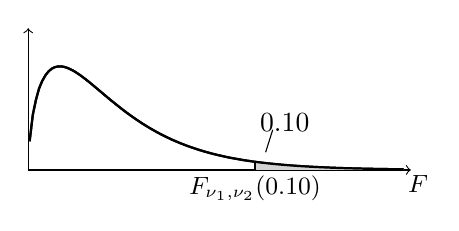
\begin{tikzpicture}[x=0.9cm,y=1.5cm]
% ---- 坐标轴 ----
\draw[->] (0,0) -- (5.4,0);
\draw[->] (0,0) -- (0,1.2);
% ---- F 分布密度曲线（近似） ----
\draw[thick,domain=0.02:5.3,samples=120]
  plot (\x,{2.6*(\x)^(0.6)*exp(-1.35*\x)});
% ---- 右侧阴影区 ----
\fill[gray!35]
  (3.2,0) -- plot[domain=3.2:5.3,samples=60]
  (\x,{2.6*(\x)^(0.6)*exp(-1.35*\x)}) -- (5.3,0) -- cycle;
\draw[thick,domain=0.02:5.3,samples=120]
  plot (\x,{2.6*(\x)^(0.6)*exp(-1.35*\x)});
% ---- 分位点竖线 ----
\draw (3.2,0) -- (3.2,{2.6*(3.2^0.6)*exp(-1.35*3.2)});
% ---- 标注 ----
\draw (3.45,0.34) -- (3.35,0.15);
\node[inner sep=1pt] at (3.62,0.40) {$0.10$};
% ---- 轴标签 ----
\node[below,inner sep=1pt,font=\small] at (3.2,-0.02) {$F_{\nu_{1},\nu_{2}}(0.10)$};
\node[below,inner sep=1pt,font=\small] at (5.5,-0.02) {$F$};
\end{tikzpicture}

{\zihao{6}
\mvfit{%
\begin{tabular}{r|*{17}{r}}
\toprule
\makecell{$\nu_{1}$\\$\nu_{2}$} & 1 & 2 & 3 & 4 & 5 & 6 & 7 & 8 & 9 & 10 & 12 & 15 & 20 & 25 & 30 & 40 & 60\\
\midrule
1 & 39.86 & 49.50 & 53.59 & 55.83 & 57.24 & 58.20 & 58.91 & 59.44 & 59.86 & 60.19 & 60.71 & 61.22 & 61.74 & 62.05 & 62.26 & 62.53 & 62.79\\
2 & 8.53 & 9.00 & 9.16 & 9.24 & 9.29 & 9.33 & 9.35 & 9.37 & 9.38 & 9.39 & 9.41 & 9.42 & 9.44 & 9.45 & 9.46 & 9.47 & 9.47\\
3 & 5.54 & 5.46 & 5.39 & 5.34 & 5.31 & 5.28 & 5.27 & 5.25 & 5.24 & 5.23 & 5.22 & 5.20 & 5.18 & 5.17 & 5.17 & 5.16 & 5.15\\
4 & 4.54 & 4.32 & 4.19 & 4.11 & 4.05 & 4.01 & 3.98 & 3.95 & 3.94 & 3.92 & 3.90 & 3.87 & 3.84 & 3.83 & 3.82 & 3.80 & 3.79\\
5 & 4.06 & 3.78 & 3.62 & 3.52 & 3.45 & 3.40 & 3.37 & 3.34 & 3.32 & 3.30 & 3.27 & 3.24 & 3.21 & 3.19 & 3.17 & 3.16 & 3.14\\
6 & 3.78 & 3.46 & 3.29 & 3.18 & 3.11 & 3.05 & 3.01 & 2.98 & 2.96 & 2.94 & 2.90 & 2.87 & 2.84 & 2.81 & 2.80 & 2.78 & 2.76\\
7 & 3.59 & 3.26 & 3.07 & 2.96 & 2.88 & 2.83 & 2.78 & 2.75 & 2.72 & 2.70 & 2.67 & 2.63 & 2.59 & 2.57 & 2.56 & 2.54 & 2.51\\
8 & 3.46 & 3.11 & 2.92 & 2.81 & 2.73 & 2.67 & 2.62 & 2.59 & 2.56 & 2.54 & 2.50 & 2.46 & 2.42 & 2.40 & 2.38 & 2.36 & 2.34\\
9 & 3.36 & 3.01 & 2.81 & 2.69 & 2.61 & 2.55 & 2.51 & 2.47 & 2.44 & 2.42 & 2.38 & 2.34 & 2.30 & 2.27 & 2.25 & 2.23 & 2.21\\
10 & 3.29 & 2.92 & 2.73 & 2.61 & 2.52 & 2.46 & 2.41 & 2.38 & 2.35 & 2.32 & 2.28 & 2.24 & 2.20 & 2.17 & 2.16 & 2.13 & 2.11\\
11 & 3.23 & 2.86 & 2.66 & 2.54 & 2.45 & 2.39 & 2.34 & 2.30 & 2.27 & 2.25 & 2.21 & 2.17 & 2.12 & 2.10 & 2.08 & 2.05 & 2.03\\
12 & 3.18 & 2.81 & 2.61 & 2.48 & 2.39 & 2.33 & 2.28 & 2.24 & 2.21 & 2.19 & 2.15 & 2.10 & 2.06 & 2.03 & 2.01 & 1.99 & 1.96\\
13 & 3.14 & 2.76 & 2.56 & 2.43 & 2.35 & 2.28 & 2.23 & 2.20 & 2.16 & 2.14 & 2.10 & 2.05 & 2.01 & 1.98 & 1.96 & 1.93 & 1.90\\
14 & 3.10 & 2.73 & 2.52 & 2.39 & 2.31 & 2.24 & 2.19 & 2.15 & 2.12 & 2.10 & 2.05 & 2.01 & 1.96 & 1.93 & 1.91 & 1.89 & 1.86\\
15 & 3.07 & 2.70 & 2.49 & 2.36 & 2.27 & 2.21 & 2.16 & 2.12 & 2.09 & 2.06 & 2.02 & 1.97 & 1.92 & 1.89 & 1.87 & 1.85 & 1.82\\
\bottomrule
\end{tabular}
}}
\end{mvtable}
